\chapter{FDM 3D PRINTERS}

\section{General Information}

Fused Deposition Modeling (FDM) is one of the most popular and widely used 3D printing technologies. Here's some general information about FDM printers:

\noindent\textbf{Principle.}
FDM printers work by heating and extruding thermoplastic filament through a heated nozzle, which deposits layers of material to build up the final object. The filament is fed from a spool into the extruder, where it is melted and extruded onto the build platform layer by layer.

\noindent\textbf{Materials.}
FDM printers can work with a wide range of thermoplastic materials, including PLA (Polylactic Acid), ABS (Acrylonitrile Butadiene Styrene), PETG (Polyethylene Terephthalate Glycol), TPU (Thermoplastic Polyurethane), and many others. Each material has its own properties in terms of strength, flexibility, temperature resistance, and surface finish.

\noindent\textbf{Build Volume.}
FDM printers are available in various sizes and configurations, with different build volumes to accommodate different project requirements. Desktop FDM printers are commonly used for prototyping, hobbyist projects, and small-scale production, while larger industrial FDM printers are used for manufacturing and production applications.

\noindent\textbf{Layer Resolution.}
FDM printers can achieve varying levels of layer resolution, ranging from coarse to fine, depending on factors such as nozzle size, layer height, and print speed. Smaller layer heights result in finer details and smoother surface finishes but may require longer print times.

\noindent\textbf{Support Structures.}
FDM printers often require support structures to be added to overhanging or bridging areas of the print to prevent sagging or collapsing during printing. These supports are typically made from the same material as the print and are removed after printing is complete.

\noindent\textbf{Post-Processing.}
After printing, FDM parts may require post-processing to improve their surface finish or mechanical properties. This can include sanding, painting, smoothing with solvents or heat, or annealing (for certain materials like ABS).

\noindent\textbf{Applications.}
FDM printers are used in a wide range of industries and applications, including prototyping, product design, manufacturing, education, healthcare, aerospace, automotive, and consumer goods. They are valued for their affordability, versatility, and ease of use.

\noindent\textbf{Open-Source Community.}
FDM printing has a vibrant open-source community that has contributed to the development of hardware, software, and materials. This community-driven approach has led to innovations in printer design, materials development, and software tools, making FDM printing more accessible and affordable for enthusiasts and professionals alike.
Overall, FDM printing is a versatile and accessible 3D printing technology that continues to evolve and expand its capabilities for a wide range of applications.


\section{Kinematic System Types}

These are just a few examples of the many kinematic systems used in 3D printers.
Each system has its own advantages, limitations, and applications, and the choice of kinematic system depends on factors such as printing speed, accuracy, build volume, and intended use.

\noindent\textbf{Cartesian.}
Cartesian 3D printers use a rectangular coordinate system with three linear axes  $(x,y,z,e)$ to move the print head and build platform.
This is the most common type of kinematic system used in desktop 3D printers.

\noindent\textbf{Delta.}
Delta printers use three vertical columns with parallel arms connected to the print head. By varying the length of the arms, the printer can precisely control the movement of the print head in three dimensions.
Delta printers are known for their fast printing speeds and are often used for tall and cylindrical prints.

\noindent\textbf{CoreXY.}
CoreXY printers use two stationary stepper motors to drive belts that move the print head along the $x$ and $y$ axes.
This configuration allows for simultaneous movement in both directions without the need for heavy motors on the moving carriage, resulting in smoother and faster motion.

\noindent\textbf{H-Bot.}
H-Bot printers use two parallel rails or tracks with a carriage that moves along each track.
The carriages are connected by a crossbeam, forming the {\textquotedblleft}H{\textquotedblright} shape.
H-Bot mechanisms allow for compact and lightweight designs, making them suitable for desktop and small-scale 3D printers.

\noindent\textbf{Scara.}
SCARA (Selective Compliance Assembly Robot Arm) printers use a robotic arm
with two parallel joints (shoulder and elbow) to control the movement of the print head.
SCARA printers are known for their speed and accuracy and are often used in industrial applications.


\noindent\textbf{Pola.}
Polar printers use a rotating build platform and a print head that moves along radial and angular axes. This configuration allows for printing objects with a cylindrical or spherical shape and is often used for specialized applications such as printing round objects or sculptures.


\section{Artillery Sidewinder X2}

The Artillery Sidewinder X2 is a 3D printer produced by Artillery, a manufacturer known for its reliable and affordable printers. The Sidewinder X2 is an upgraded version of the original Sidewinder, boasting several improvements and enhancements.

Some key features of the Artillery Sidewinder X2 include:

\noindent\textbf{Large Build Volume.}
It offers a spacious build volume, allowing users to create relatively large 3D prints compared to many other printers in its price range.

\noindent\textbf{Dual $Z$-Axis.}
The Sidewinder X2 features a dual $Z$-axis design, which helps in ensuring more stable and precise vertical movement during printing, resulting in improved print quality.

\noindent\textbf{Direct Drive Extruder.}
It utilizes a direct drive extruder system, which is known for better filament control and compatibility with a wider range of filament types,
including flexible materials.

\noindent\textbf{Touchscreen Interface.}
The printer is equipped with a touchscreen interface, making it easy to navigate and control various settings and functions.

\noindent\textbf{Fast Printing Speed.}
It is capable of printing at relatively high speeds while maintaining print quality,
thanks to its robust construction and efficient design.

\noindent\textbf{Silent Printing.}
The Sidewinder X2 is known for its relatively quiet operation,
which is achieved through the use of high-quality stepper motors and other noise-reducing components.

Overall, the Artillery Sidewinder X2 is popular among 3D printing enthusiasts and hobbyists for its combination of large build volume,
reliable performance, and affordable price point.

\begin{figure}[h!tb]
\centering
\begin{multicols}{3}
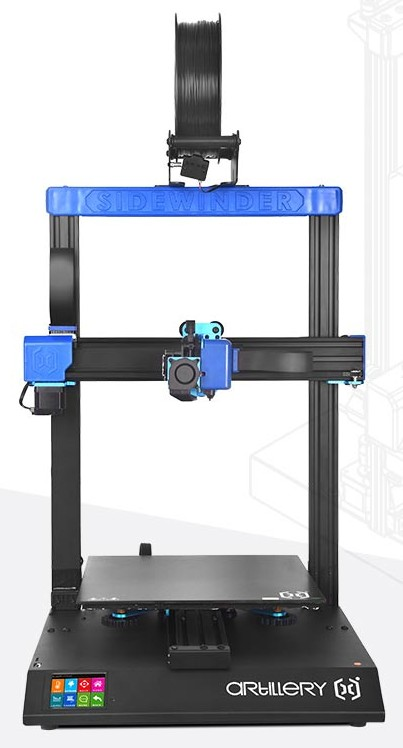
\includegraphics[scale=0.20]{x2-f1-edited.jpg}\par
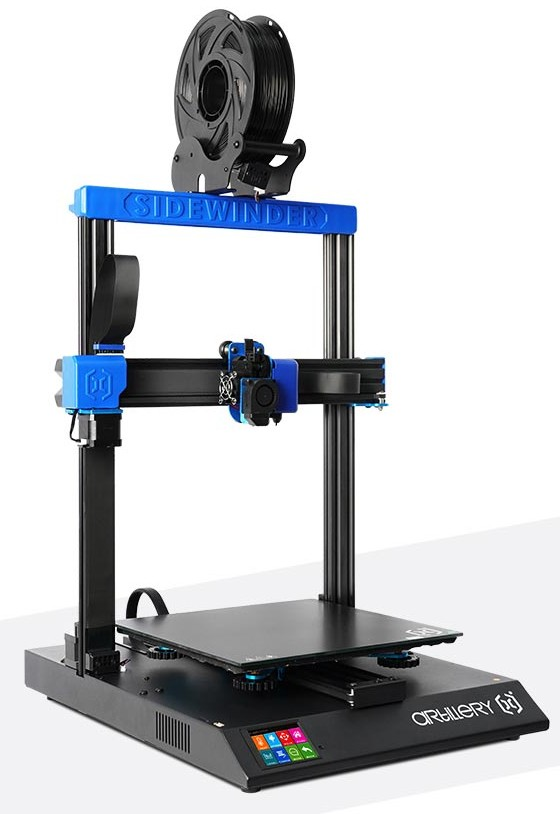
\includegraphics[scale=0.20]{x2-f2-edited.jpg}\par
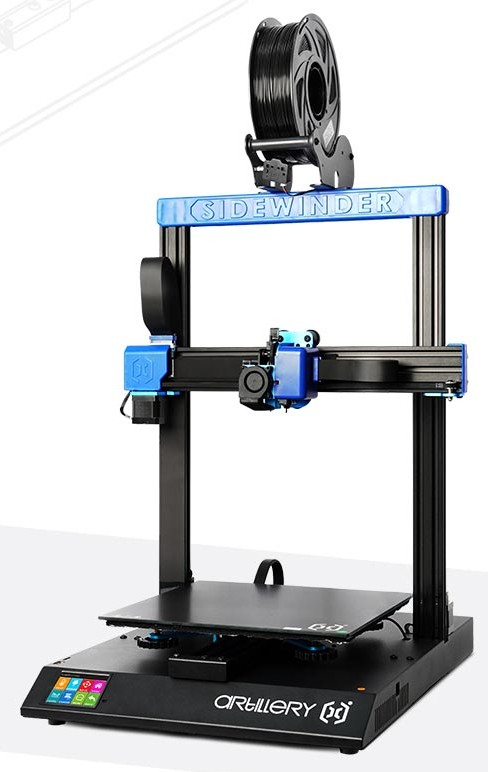
\includegraphics[scale=0.20]{x2-f3-edited.jpg}
\end{multicols}
%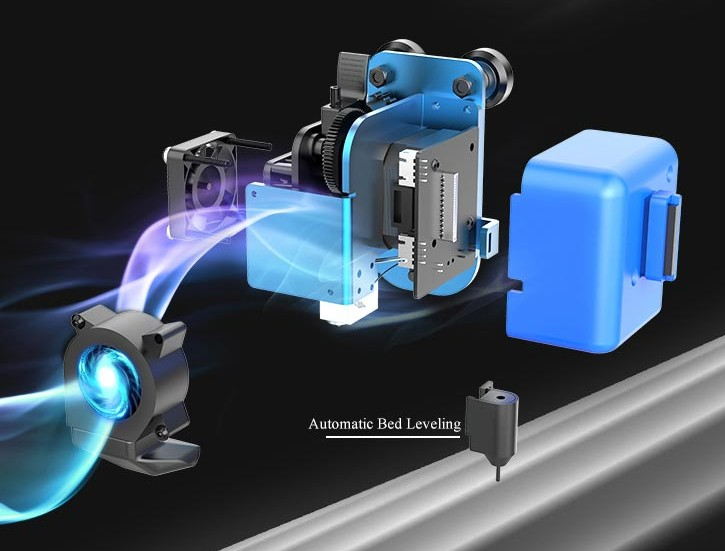
\includegraphics[scale=0.15]{x2-e-edited.jpg}
\caption{Artillery Sidewinder X2}
\label{fig:label1}
\end{figure}

\begin{figure}[h!tb]
\centering
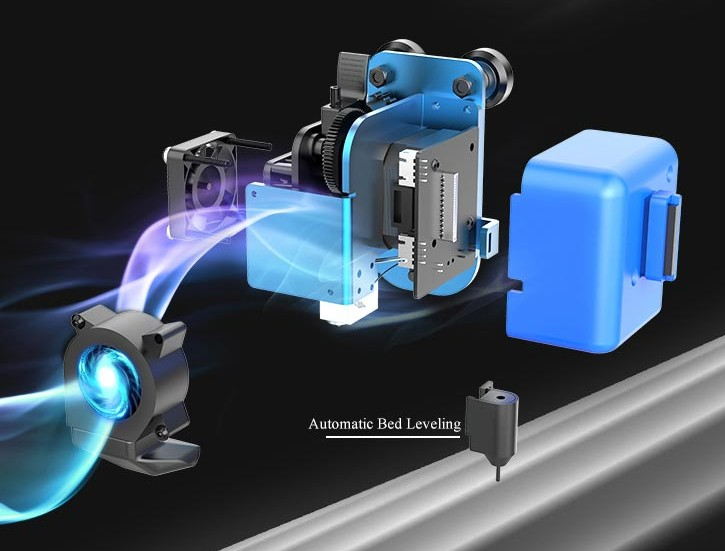
\includegraphics[scale=0.40]{x2-e-edited.jpg}
\caption{Artillery Sidewinder X2 - Extruder}
\label{fig:label2}
\end{figure}


%\noindent örnek tablo.
%
%\begin{table}[h]
%	\centering
%		\begin{tabular}{cccc}
%			\hline\hline
%			$ N $   & $ n=3 $ & $ n=4 $ & $ n=5 $ \\
%			\hline
%			20/40   & 1.69    & 2.86    & 3.88    \\
%			40/80   & 1.88    & 2.94    & 3.94    \\
%			80/160  & 1.95    & 2.97    & 3.99    \\
%			\hline\hline
%		\end{tabular}
%	\caption{Bla bla bla...}\label{tab:label}
%\end{table}
%
%\section{Section başlığı 2}
%\subsection{SubSection örneği}
%Citetion örneği: \cite{allaire2008numerical}.

